\documentclass[12pt, a4paper]{article}

\usepackage[T1]{fontenc}
\usepackage[utf8]{inputenc}
\usepackage{amsmath, amssymb, amsfonts, amsthm}
\usepackage{bbm}
\usepackage{graphicx}
\usepackage{verbatim}
\usepackage{caption}
\usepackage{subcaption}
\usepackage{subfig}
\usepackage{float}
\usepackage{algorithm}
\usepackage{algpseudocode}

\theoremstyle{definition}
\newtheorem*{definition}{Teorem}

\newcommand{\vb}{\mathbf}

\renewcommand{\contentsname}{Innhald}

\renewcommand{\abstractname}{Samandrag}

\renewcommand{\figurename}{Figur}

\makeatletter
\newcommand{\newalgname}[1]{
    \renewcommand{\ALG@name}{#1}
}
\newalgname{Algoritme}

\begin{document}

\begin{titlepage}
    \begin{center}
        \vspace*{1cm}
        
        \textbf{\huge Molekylær Dynamikk}

        \vspace{0.5cm}
        \textbf{Oblig 3}

        \vspace{1.5cm}
        \textbf{Øyvind Sigmundson Schøyen} \\
        Kandidatnummer: 30 \\

        \vspace{1.5cm}

        Avsluttande prosjekt i FYS3150 \\

        \vspace{3.0cm}

        \includegraphics[width=0.4\textwidth]{\string~/Downloads/UiO_Segl_300dpi.png}

        \vspace{1.0cm}

        FYS3150 Computational Physics\\
        Universitetet i Oslo\\

        \vfill

        1. desember 2014

    \end{center}
\end{titlepage}

\begin{abstract}
    I dette prosjektet har me tatt for oss modellering av argon på atomært nivå. Me har vore interesserte i å lage eit program som skal lage ein atomstruktur etter eige ynskje.
    I tillegg har me ville sjå på korleis eit slikt system utvikler seg over tid og måle statistiske eigenskapar ved det. For å modellere eit så realistisk resulatat innenfor
    det som er mogleg å køyre på ein pc har me utnytta cellelister for å auke hastigheita på programmet. For krafta har me nytta Lennard Jones potensialet og som integrator
    har me brukt Velocity Verlet-algoritma. Programma våre er objektorienter C++-kode med eit Python rammeverk som skal enklast mogleg køyre programmet vårt for forskjellige 
    parametrar og plotte verdiar. Me nyttar VMD for å visualisere atoma i rommet. All kjeldekode ligg på github.\\ \\
    Rett litt på denne\dots \\ \\
    \texttt{https://github.com/Schoyen/molecular-dynamics-fys3150}
\end{abstract}

\newpage
    \tableofcontents
\newpage

\section*{Introduksjon}
    \addcontentsline{toc}{section}{Introduksjon}
    Oppgåva me er gjevne har gått ut på å modellere eit fysisk system samt bruke objektorientert programmering til å holde ein ryddig, oversiktlig, samt effektiv kode. 
    I byrjinga er me gjeve ein kode som lagar 100 argon atom og gjer dei ein tilfeldig retning og hastighet. Gjeve lang nok tid vil atoma drive vekk. Me vil difor nytte
    ``periodiske randbetingelsar'' for å halde atoma i nærleiken. Grunna hastigheitar gjevne frå Maxwell-Bolzmann distribusjon vil systemet ha ein ikkje-null
    rørslemengde som me vil fjerne. Me vil deretter lage ein krystallstruktur kor me startar simuleringa av atoma. I eit slik lukka system vil total energien vere bevart, 
    men grunna numerisk avrunding er det ikkje alltid dette held mål. Ein stabil alogritme som me vil nytte er ``Velocity Verlet'' som er ein symplektisk integrator. % Forklar dette.
    Me vil no byrje å måle statistiske eigenskapar som energi og temperatur. For å kunne køyre koden for store system vil me derimot utvikle ein kjappar algoritme når 
    me rekner ut krafta mellom atompara. Dette løyser me med cellelister. Til slutt, i fyrste del av prosjektet, legg me til ein termostat som let oss kontrollere 
    temperaturen i systemet. \\ \\
    % Fyll in for del 2 av prosjektet.
    God lesning!



\newpage


\section*{Fysikken bak molekylær dynamikken}
    \addcontentsline{toc}{section}{Fysikken bak molekylær dynamikken}
    I denne delen av rapporten vil me sjå på dei forskjellige eigenskapane me måler i MD-koda vår. Eventuelle måleresultat vil bli vist i resultat-seksjonen.

    \subsection*{Oppsett}
        \addcontentsline{toc}{subsection}{Oppsett}
        Systemet med atom me set opp krev nokre tilpassningar for å gje eit realistisk resultat. 

        \subsubsection*{Face-Centered Cubic Lattice}
            \addcontentsline{toc}{subsubsection}{Face-Centered Cubic Lattice}
            Det fyrste me vil gjere å plassera atom i ein krystallstruktur. For Argon
            vil me då nytte ``face-centered cubic lattice'' (FCC). Me plasserer fire og fire atom i ei einingscelle. Posisjonane til kvart atom vil vere gjeve ved
            \begin{align*}
                &\vb{r}_1 = 0\vb{i} + 0\vb{j} + 0\vb{k}, \\
                &\vb{r}_2 = \frac{b}{2}\vb{i} + \frac{b}{2}\vb{j} + 0\vb{k}, \\
                &\vb{r}_3 = 0\vb{i} + \frac{b}{2}\vb{j} + \frac{b}{2}\vb{k}, \\
                &\vb{r}_4 = \frac{b}{2}\vb{i} + 0\vb{j} + \frac{b}{2}\vb{k}.
            \end{align*}
            Her vil $b$ vere ein konstant, me skal seinare sjå på korleis trykket er avhengig av denne. \\ % Hugs å legg dette ved i resultatet.

        \subsubsection*{Maxwell-Boltzmann og fartsmoment}
            \addcontentsline{toc}{subsubsection}{Maxwell-Boltzmann og fartsmoment}
            Etter at atoma vert plasserte i einingscellene vil me gje dei ein liten starthastighet kor me nyttar Maxwell-Boltzmann distribusjon. Då vil
            \begin{align*}
                \vb{v} \propto \sqrt{T}.
            \end{align*}
            Hastigheita til atoma vil bli fordelte tilfeldig i rommet. Resultatet er at systemet har eit ikkje-null fartsmoment. Før me byrjar å rekne ut nye posisjonar vil
            me fjerne dette fartsmomentet. Me vil då finne den totale hastigheita til systemet og trekke denne frå kvart atom.
            \begin{align*}
                &\vb{V} = \frac{1}{M}\sum_i^N m_i\vb{v}_{i}^{\text{før}}, \\
                &\vb{v}_{i}^{\text{etter}} = \vb{v}_{i}^{\text{før}} - \vb{V}, \qquad \ i \in [1, N],
            \end{align*}
            kor $\vb{V}$ er den total hastigheita til systemet, $N$ er antal atom, $M$ er den totale massa til alle atoma summert opp. Dette bidrar til at systemet vårt
            ikkje har ein total hastigheit, men heller står i ro. \\



        \subsubsection*{Lennard Jones}
            \addcontentsline{toc}{subsubsection}{Lennard Jones}
            For å få ein fysisk effekt på systemet må me byrje å rekne ut krafta mellom atoma. Me nyttar Lennard Jones potensialet for å finne krafta mellom atompara.
            Lennard Jones har den eigenskapen at potensialet tek med den fråstøytande og den tiltrekkande krafta mellom para. Potensialet er gjeve ved
            \begin{align*}
                U(r_{ij}) = 4\epsilon\left[ \left( \frac{\sigma}{r_{ij}} \right)^{12} - \left( \frac{\sigma}{r_{ij}} \right)^{6} \right],
            \end{align*}
            kor $r_{ij}$ er avstanden frå atom $i$ og $j$, $\sigma$ og $\epsilon$ er konstantar som bestemmer kva distanse potensialet er null og kor djup potensialbrønnen skal vere.
            Me finn krafta ved å ta den negative gradienten til potensialet. Då får me
            \begin{align*}
                \vb{F}(\vb{r}_{ij}) &= -\nabla U(r_{ij}) = -\frac{\partial U(r_{ij})}{\partial r_{ij}} \\
                &= -4\epsilon\left[ 12\left( \frac{\sigma^{12}}{r_{ij}^{14}} \right) - 6\left( \frac{\sigma^6}{r_{ij}^8} \right) \right]\vb{r_{ij}}.
            \end{align*}
            Grunna dei høge potensane kan me sjå at denne krafta vil kjapt gå mot null. Denne eigenskapen gjer at me kan effektivisere koda vår ved berre å rekne ut krafta 
            mellom atom kor avstanden mellom dei er innenfor ein radius $r_{\text{cut}}$.
            Eit plott over $U/\epsilon$ mot $r_{ij}/\sigma$ vil gje oss ein indikator kva tid krafta vil vere null.
            \begin{figure}[H]
                \centering
                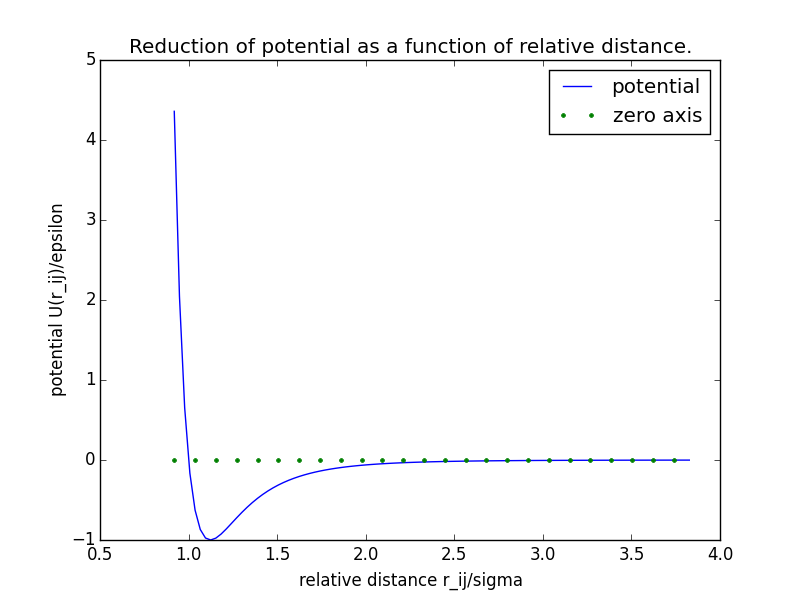
\includegraphics[width=400px]{potentialPlot.png}
                \caption{I plottet kan me lett sjå kor dei tiltrekkjande og kor dei fråstøytande kreftene har sine styrker. Då krafta er gjeve som den negative gradienten til
                        potensialet vil me kunne sjå at i det atoma kjem veldig nære einannan vil det virke ei kraftig fråstøyting ($r_{ij}^{12}$-delen) medan det for større avstand
                        vil virke ei svakare, men med større rekkevidde, tiltrekkande kraft ($r_{ij}^6$-delen).}
            \end{figure}
            Frå figuren les me av 
            \begin{align*}
                \frac{r_{\text{cut}}}{\sigma} \approx 2.5 \qquad \Rightarrow \qquad r_{\text{cut}} \approx 2.5\sigma.
            \end{align*}
            Utanfor denne radiusen vil me ikkje rekne krafta mellom atompara.


    \newpage

    \subsection*{Statisiske målingar}
        \addcontentsline{toc}{subsection}{Statistiske målingar}
        Hensikten med koda vår er for å måle eigenskapar i eit system med atomar.

        \subsubsection*{Energi}
            \addcontentsline{toc}{subsubsection}{Energi}
            Det enklaste å måle vil vere energien i systemet. Me har allereie implementert eit uttrykk for den potensielle energien med Lennard Jones. Då finner me
            den kinetiske energien ved formelen
            \begin{align*}
                E_{k} = \sum_{i}^N\frac{1}{2}m_iv_{i}^2,
            \end{align*}
            kor $N$ er antal atomar i systemet. Total energien vil då vere gjeve ved
            \begin{align*}
                E = E_{k} + U.
            \end{align*}
            For eit system av atom med dei randbetingelsane me har satt forventer me energibevaring. Grunna numerisk avrunding vil det alltid oppstå små fluktuasjonar,
            men desse forventer knapt skal vere synlege. \\

            Då me ikkje reknar krafta mellom atompar utanfor $r_{\text{cut}}$ må me endre litt på Lennard Jones potensialet slik at me har energibevaring. 
            Potensialet vil nå bli skalert etter likninga
            \begin{align*}
                U_{\text{skalert}}(r_{ij}) = 
                \begin{cases}
                    U(r_{ij}) - U(r_{\text{cut}}), & r \leq r_{\text{cut}} \\
                    0, & r > r_{\text{cut}}.
                \end{cases}
            \end{align*}

        \subsubsection*{Temperatur}
            \addcontentsline{toc}{subsubsection}{Temperatur}
            Temperaturen speler ei stor rolle i systemet vårt. Me er interesserte i å finne ut kva tid strukturen smelter og kor tid ho held seg stabil. Me finn ho 
            ved ekvipartisjonsteoremet som seier
            \begin{align*}
                &\left \langle E_{k} \right \rangle = \frac{3}{2} = Nk_{B}T, \\
                &\Rightarrow T = \frac{2}{3}\frac{E_{k}}{Nk_{B}},
            \end{align*}
            kor $T$ då angjer den momentane temperaturen då me ikkje tek gjennomsnittet av $E_{k}$. Temperaturen vil fluktuere då den kinetiske energien vil endre seg for
            kvart tidssteg. Etterkvart vil me nå eit stabilt likevektspunkt kor temperaturen held seg nokonlunde jamnt.


        \subsubsection*{Berendsen termostat}
            \addcontentsline{toc}{subsubsection}{Berendsen termostat}


\newpage


\section*{Algoritmar}
    \addcontentsline{toc}{section}{Algoritmar}

    \subsection*{Simulering av eit uendeleg stort system}
        \addcontentsline{toc}{subsection}{Simulering av eit uendeleg stort system}
        Då me ikkje kan simulere eit uendeleg stort system vil me nytte nokre metodar kor me slepper å sjå at atoma våre forsvinn ut i ingenting.

        \subsubsection*{Periodiske randbetingelsar}
            \addcontentsline{toc}{subsubsection}{Periodiske randbetingelsar}
            Viss eit atom har ein 
            posisjon som ligg utanfor storleiken på systemet vårt vil me flytte atomet slik at det kjem inn frå den andre sida av systemet. For eit stort system kan dette 
            vere ei god tilnærming då det heile tida forsvinn atom ut frå eit lite område, men samstundes kjem det inn nye atom slik at tettheten er jamn. Dette vil og vere med
            på å gje oss bevaring av total energi då det ikkje går noko tap til vegger og liknande. Periodiske randbetingelsar vil vere gjeve ved formelen
            \begin{align*}
                \vb{r}_i = x_i\vb{i} + y_i\vb{j} + z_i\vb{k}, \qquad i \in [1, N],
            \end{align*}
            kor $N$ er antal atom i systemet. Då vil kvar komponent i $\vb{r}_i$ vere gjeve ved
            \begin{align*}
                x = 
                \begin{cases}
                    x + S_x, & x < 0 \\
                    x, & x \in [0, S_x) \\
                    x - S_x, & x \geq S_x
                \end{cases},
            \end{align*}
            kor $S_x$ er storleiken på systemet i $x$-retning og $x$ er noverande posisjon for atomet. Me gjentek dette for dei to andre retningane og.



        \subsubsection*{Avstand frå endepunkta}
            \addcontentsline{toc}{subsubsection}{Avstand frå endepunkta}
            Frå analogien ved bruk av periodiske randbetingelsar må me ta hensyn til at avstand mellom atompar ikkje nødvendigvis stemmer. Argumentet vårt er at 
            atoma som ligg heilt i kanten av systemet har ``tvillingar'' som kjem inn frå andre sida på nøyaktig same tid og med dei same parametrane som seg sjølve.
            Når me då rekner avstand mellom atoma vil me sjekke om eigentleg ligg mykje nærare viss det eine atomet vert flytta over på den andre sida av systemet.
            Me kjem til å nytte ``Minimum Image Criterion'' for å sjekke om dette er oppfylt. Me definerer
            \begin{align*}
                \Delta \vb{R} = \vb{r}_i - \vb{r}_j, \qquad i \neq j, \qquad i, j \in [1, N],
            \end{align*}
            som gjer oss avstanden mellom atoma slik det framstår i simuleringa. For å simulere eit uendeleg system vil me difor sjekke om denne oppfyller krava
            \begin{align*}
                \Delta \vb{R} = \Delta X\vb{i} + \Delta Y\vb{j} + \Delta Z\vb{k},
            \end{align*}
            kor me har skrive $\Delta \vb{R}$ på komponentform. Då får me
            \begin{align*}
                \Delta X = 
                \begin{cases}
                    \Delta X - S_x, & \Delta X > \frac{S_x}{2} \\
                    \Delta X, & \Delta X \in \left( -\frac{S_x}{2}, \frac{S_x}{2} \right] \\
                    \Delta X + S_x, & \Delta X \leq -\frac{S_x}{2}
                \end{cases}
            \end{align*}




    \subsection*{Velocity Verlet}
        \addcontentsline{toc}{subsection}{Velocity Verlet}
        Idet systemet vårt er satt opp med ein starthastighet for kvart atom vil me tidsintegrere oss fram i tid for å sjå korleis det utvikler seg. Då systemet vårt er pakka
        inn med periodiske randbetingelser og biletekriterie vil me nytte ein algoritme som bevarer energien. Velocity Verlet er ein $\textbf{symplektisk integrator}$ som 
        bevarer total energien (Hamiltonian er bevart, men denne tilsvarer ofte total energien i eit system). Velocity Verlet er i tillegg ein enkel og kompakt algoritme med
        eit feilledd som går som $\mathcal{O}(\Delta t^2)$. Integrasjonen består av tre ledd
        \begin{align*}
            \vb{v}(t + \Delta t/2) &= \vb{v}(t) + \frac{\vb{F}(t)}{m}\frac{\Delta t}{2}, \\
            \vb{r}(t + \Delta t) &= \vb{r}(t) + \vb{v}(t + \Delta t/2)\Delta t, \\
            \vb{v}(t + \Delta t) &= \vb{v}(t + \Delta t/2) + \frac{\vb{F}(t + \Delta t)}{m}\frac{\Delta t}{2},
        \end{align*}
        kor me må rekne ut krafta ein gong for fyrste ledd før me byrjar å integrere oss fram i tid.

    \subsection*{Cellelister}
        \addcontentsline{toc}{subsection}{Cellelister}
        Det som er kostbart ved Velocity Verlet er utrekninga av kraft to gonger per ledd. Viss me rekner ut krafta mellom kvart atom vil me ha ei algoritme som går som
        $\mathcal{O}(N^2)$, kor $N$ er antal atom. Ved å sette opp cellelister vil me dele opp systemet vårt i mindre celler kor kvar side av cellene har lengde 
        $r_{\text{cut}}$ runda av til næraste heiltal. Ved å gjere dette slipper me å leite gjennom alle atoma i systemet vårt og rekne ut krafta mellom dei. Me vil 
        heller rekne ut krafta mellom atoma i ei celle og alle nabocellene til denne cella. Viss me då i tillegg sjekker om atoma i nabocellene ligg utanfor
        $r_{\text{cut}}$ vil me redusere køyretida til $\mathcal{O}(N)$.

        \begin{algorithm}[H]
            \caption{Rekn ut krafta ved hjelp av cellelister}
            \label{Cellelister}
            \begin{algorithmic}[1]
                \For {$i \in N_x$}
                    \For {$j \in N_y$}
                        \For {$k \in N_z$}
                            \State $Cell_{1} = CellIndex(i, j, k)$
                            \For {$cx \in \left[ i - 1, i + 1 \right]$}
                                \For {$cy \in \left[ j - 1, j + 1 \right]$}
                                    \For {$cz \in \left[ k - 1, k + 1 \right]$}
                                        \State $applyPeriodic(cx, cy, cz)$
                                        \State $Cell_{2} = CellIndex(cx, cy, cz)$
                                        \For {$m \in Cell_1.getAtoms()$}
                                            \For {$n \in Cell_2.getAtoms()$}
                                                \State Rekn ut krafta
                                            \EndFor
                                        \EndFor
                                    \EndFor
                                \EndFor
                            \EndFor
                        \EndFor
                    \EndFor
                \EndFor
            \end{algorithmic}
        \end{algorithm}
        Her er $N_x$, $N_y$ og $N_z$ antal celler i henholdsvis $x$-, $y$- og $z$-retning. $cx$, $cy$ og $cz$ viser til koordinatane til nabocellene. Metoden $applyPeriodic()$ 
        sjekker om cellene i endepunkta har naboar på andre sida av systemet. \\
        For kvart tidssteg må me legge atom i dei riktige cellene. Me lagrar cellene på indeksar gjeve ved formelen
        \begin{align*}
            index = iN_yN_z + jN_z + k,
        \end{align*}
        kor $i$, $j$ og $k$ er indeksane me sender inn. Då kan me finne kva celle eit atom høyrer til i ved å nytte formelen
        \begin{align*}
            index_x = \left \lfloor \frac{x_{\text{Atom}}}{S_{x}} N_{x}\right \rfloor,
        \end{align*}
        og tilsvarande for $y$- og $z$-retning. Då vil $index$-formelen over returnere cella som inneheld det gjeldane atomet.

\newpage
\section*{Struktur}
    \addcontentsline{toc}{section}{Struktur}




\newpage


\section*{Resultat}
    \addcontentsline{toc}{section}{Resultat}

    % Hugs å sjå på bevaring av energi for forskjellige val av dt.
    % Legg ved smeltetemperatur og stabilitetstemperatur.
    % Sjå på kvifor temperaturen synker og korleis fluktuasjonar avhenger av antal atom.



\newpage


\section*{Feilestimat}
    \addcontentsline{toc}{section}{Feilestimat}
\end{document}
